\documentclass{article}

\usepackage[T1]{fontenc}
\usepackage[utf8]{inputenc}
\usepackage{mdwlist} % To have compact lists
\usepackage{hyperref} % To have links to URLs
\usepackage{float} % To force images to the right place
\usepackage{listings} % To display source code

\usepackage{caption}
\usepackage{subcaption}


% To include images
\usepackage{graphicx} 
\graphicspath{ {images/} } % location of images

% To adjust image position
\usepackage[export]{adjustbox}

% To add hyperlink
\usepackage{hyperref}

% Disables automatic indents globally
%\setlength{\parindent}{0pt}

% Set link color to blue
\hypersetup{
    colorlinks=true,
    linkcolor=blue,
    filecolor=blue,      
    urlcolor=blue,
    citecolor=blue
}

%
% Quality of Writing & Organisation of Document
% 
% Weight: 20/90 = 22%
%
% Grades:
%   A+ to B-:
%		Very well written document (well organised, good layout, good English, 
%		and clarity in writing).
%   C+ to D-:
%		Well organised and written but some issues in language, the flow of the 
%		document, references, etc.
%   E+ to G:
%		Badly prepared document (poor organisation, poor layout, sloppy English, 
%		and lack of clarity in writing).
%

\begin{document}

% - - - - Header Begins - - - -
\begin{center}
	{\LARGE \textbf{Interim Report}} \\
	\vspace{0.5em}
	\textsl{Team $\lambda$ Lovelace}
\end{center}

\vspace{0.5em}

\begin{center}
	24th June 2016 \\
	COMP47250, Team Software Project 2016 \\ 
	University College Dublin, Ireland \\
\end{center}

\vspace{0.5em}
% - - - - Header Ends - - - -

% Executive summary
%\renewcommand{\abstractname}{Executive Summary}
%\begin{abstract}
%\noindent A collaborative recommender system for tweets; a more personalised tweet stream.
%\end{abstract}


\noindent This is an interim project report on the Minimum Viable Product (MVP) for the team $\lambda$ Lovelace, summer 2016. The module formally started 2016.05.16 and will end in a final code \& report submission on 2016.08.19. This document was submitted six weeks after the start of the project.
\\\\
The purpose of this report is:

\begin{itemize*}
    \item To give an overall picture of the project vision
    \item To demonstrate the progress made to date
    \item To build confidence in a plan for project completion
\end{itemize*}

\noindent It is assumed the reader is familiar with Twitter. If not, there is a short appendix at the end of this document detailing a few of the main features.


%==============================================================================
\section{User Scenario: The Characters}
% 500 words, weight: 10/90 = 11%
%
% * Who is your target user?
% * Why are they important?
% * What problem are you solving for them?
%
% Grades:
%   A+ to B-:
%		Very well defined user scenario and problem with strong links between 
%		the two.
%   C+ to D-:
%		Well defined user scenario and problem (maybe missing connections 
%		between the two, or importance of problem not convincing).
%    E+ to G:
%		Poorly defined user scenario and problem.
%
Users of the $\lambda$ Lovelace system and the problems it solves.

\subsection{Who are your potential users?}
\begin{itemize*}
    \item Power users - this is an active Twitter user who follows more than 100 accounts. Their twitter home timeline is populated with approximately 200 tweets per day and they tweet, retweet or like approximately five times daily.
    \item Regular users - a user who is not very active and tweets roughly once a week. This user follows about 50 accounts.
    \item Non-power users - a user who uses Twitter rarely.
\end{itemize*} 


\includegraphics[width=0.6\textwidth, center]{twitter_power_user}

\subsection{Why are they important?}
The system mainly targets power users, rather than the latter two categories. The power user has many tweets passing through their timeline every day and regularly engages in conversations on Twitter. These users compose a significant portion of the Twitter userbase, so it is important that they have the best possible experience when using Twitter. These users are also the most prone to the relevancy issue that plagues Twitter, which the $\lambda$ Lovelace system aims to combat.
As the recommender system's main focus is on filtering out the users home timeline of irrelevant tweets, the recommender system is most applicable to a power user. A regular user has a Twitter timeline where there is not enough activity to warrant a recommender system. They will likely see most of the news and tweets that they are interested in, along with irrelevant tweets. There is not enough volume in the normal users timeline for the irrelevant tweets to affect their Twitter experience.

\subsection{What problem are you solving for them?}
The main issue that this project will solve arises when there is an overabundance of tweets.
\\\\
\noindent The following are two problem scenarios that twitter users currently face:

\begin{itemize*}
	 \item The users Twitter timeline showing irrelevant tweets.
	 \item The users relevant tweets being lost in the bulk of irrelevant tweets.
\end{itemize*}

\subsubsection*{Problem One Scenario/Solution}
In this scenario, there is an active twitter user "Robert" who works for a software development company using Microsoft Technology. He follows Scott Hanselman, a principal program manager from Microsoft, for interesting updates in Microsoft Technology. Scott Hanselman is also diabetic and posts tweets related to diabetes. Robert, who is 22 years old and not diabetic, may not be interested in Scott's diabetes related tweets. The recommender system will personalise Robert's timeline by prioritising relevant tweets, such as Scott Hanselmans technology related tweets, and filtering out his diabetes related tweets. In essence, this means that the system is prioritising only the relevant content of a twitter account while de-prioritising the less relevant.

\subsubsection*{Problem Two Scenario/Solution}
Robert may follow many others who tweet on myriad topics. Due to the issues described in scenario one, the user must sift through many irrelevant tweets before reaching an occasional tweet that they are interested in. As the recommender system orders tweets by relevancy, there is far less of a chance that Robert will miss out on tweets in which he has a strong interest.


%==============================================================================
\section{Technical Problem}
% 1000 words, weight: 20/90 = 22%
%
% * Why does your system exist?
% * What is the core technical problem?
% * Can you describe the problem graphically?
% * Can you review other existing systems or products that address this 
%   problem? (how do they meet or fail to meet the needs of your target 
%   users)
%
% Grades:
%   A+ to B-:
%		Very clear definition of the key technical challenges involved in 
%		building the proposed system, tightly linked to the user scenario 
%		described. Also good assessment of existing similar systems.
%   C+ to D-:
%		Reasonable description of technical problem and current state of the 
%		art, but lacking in some ways. Perhaps the technical problems are 
%		described at much too low a level (“writing this function will be 
%		hard”), technical problems do not relate to the user scenario described 
%		or coverage of existing systems is limited.
%    E+ to G:
%		Inability to identify the technical challenges in addressing the user 
%		problem described in the previous section.
%

\subsection{Purpose}
% Sophie: instead of saying "the issues brought up in the User Scenario section",  I would quickly restate what those issues are. It would read: "to tackle ______".
The $\lambda$ Lovelace project was created in order to tackle the issue of irrelevant tweets being shown in the timeline, and relevant tweets being overshadowed by irrelevant tweets. Twitter is not a segmented source of information and news, but comprises of people with a multitude of opinions from many diverse backgrounds. As a form of social media, its users are encouraged to give their opinions on current events, aspects of their background and their profession. Twitter itself stirs up discussion on current events with the use of hashtags, further promoting diverse conversations. All of this activity creates a very noisy environment, which makes it difficult for the user to access the tweets that are the most relevant to their interests. For example, the User Scenario section describes how Scott Hanselman discusses and promotes news on diabetes. His account also discusses his home life, children and other personal matters. This is likely due to the social media aspect of Twitter. 

However, the average user may not always be interested in reading tweets that are not directly related to their interests. For example, Andrew Clark recently tweeted the following\cite{clark1}:

\begin{figure}[H]
    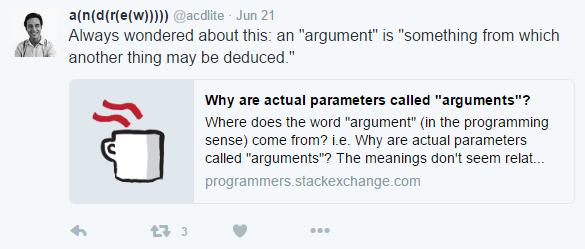
\includegraphics[width=0.6\textwidth, center]{clark1}
\end{figure}

Then shortly followed up with a political tweet, a subject completely unrelated to programming\cite{clark2}:

\begin{figure}[H]
    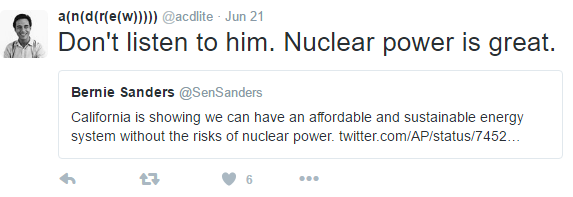
\includegraphics[width=0.6\textwidth, center]{clark2}
\end{figure}

\subsection{Core Technical Problem}

The core technical problem for this project is recommending more relevant tweets to the user first, while demoting the least relevant tweets to appearing later. This is based entirely on the user's own interests on Twitter. The Andrew Clark tweets shown above are an example of how divided a Twitter account's content can be. Only software developers, or those with an interest in technology, should see the former tweet.

% Sophie: as a non-technical person, I don't really follow this, especially why it's necessary to use the Twitter API, which seems like an important thing to understand.
In order to create a system that provides such recommendations, this project must use the Twitter REST API. However, there are rate limits placed on how many tweets can be extracted from the REST API at a time. Specifically, a user of the REST API may make 180 requests for a maximum of 3200 tweets every fifteen minutes for the user timeline. For the home timeline, a user of the API may only make fifteen requests for a maximum of 800 tweets every fifteen minutes. 

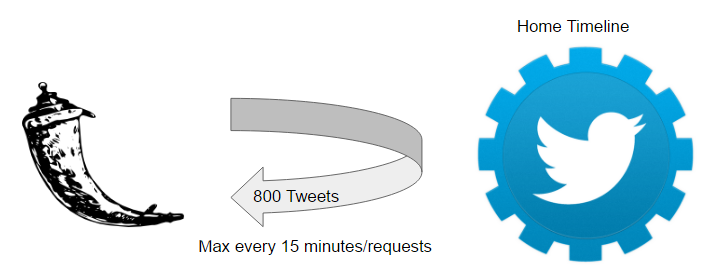
\includegraphics[width=0.6\textwidth,center]{rate_limit_1}

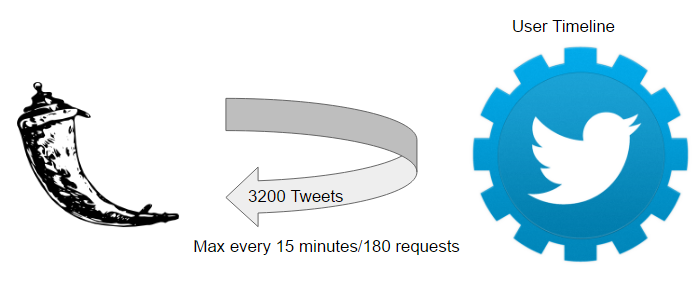
\includegraphics[width=0.6\textwidth,center]{rate_limit_2}

In both cases, this only applies to the most recent tweets. The project will also use the User Streams API, which terminates older connections as newer connections are created. The documentation does not specify how many connections are required to breach this limit, and the project is not currently at the point where such limitations can be tested.

These limitations will also require the system to store tweets as it requires a history of tweets from the user in order to build the users term-frequency document. Initially, the API can only return 800 tweets for the user. After this, the User Stream is used to constantly request the users home timeline tweets as they come in. Once the user logs back in, or fifteen minutes has passed, a request is made to the document database for a list of recommended tweets, which are obtained through automated Celery\cite{celery} jobs. Once they have read all of these tweets, the User Stream is used again.

\subsection{Competitors}

% Sophie: I think you're missing some information on what your competitors don't provide that Lamda Lovelace can.

\subsubsection*{The Official Twitter mobile app}
This app is the official mobile offering from Twitter for their system. It performs similarly to the main website, but includes the option of providing tweet recommendations. This was discovered by the team in week two. It is seemingly allowed to access the Twitter API without the same restrictions as third-party apps. This app also has access to a set of personalised recommendations, which it is assumed comes from the API. Bearing all of this in mind, the Official Twitter mobile app is currently this project's main competitor. While it is a strong competitor, it also suggests many irrelevant tweets to the user as well as advertisements.

\subsubsection*{Flipboard}
Flipboard is a social news aggregator that provides personalised news article recommendations to the user, but is not a direct competitor to $\lambda$ Lovelace as it is not solely reliant on twitter for its content. It does however, still provide personalised recommendations on the iOS platform, albeit mainly for news articles. Flipboard provides a novel solution to the cold-start problem by suggesting a broad topic preference to the user when they first log in. When selected, these topics  are in-turn used to suggest more narrow-focused aspects of that topic as a new topic. This process allows Flipboard to eventually narrow down the users interests to very specific aspects of a broad subject. For example, research for this app has shown that it is possible to narrow down from the broad category of “technology”, to the more specific term “agile development” upon initial setup of the app. Once the app was running, it shortly suggested “JavaScript”.

\subsubsection*{News360}
News360 is another social news aggregator, very similar to Flipboard that also focuses on news articles from large publishers. However, where Flipboard asks for general topics to indicate preference,  News360 requires users to vote with a thumbs up/down option. This is somewhat similar to $\lambda$ Lovelace's like/dislike functionality for tweets. News360 also provides summaries of their articles, although this summarisation of news does not apply to the $\lambda$ Lovelace project. Its cold-start solution also allows users to “love” topics, as well as like them. This allows for further emphasis on topics that strongly interest the user.

%==============================================================================
\section{Technical Solution}
% 1000 words, weight: 20/90 = 22%
%
% * What does your system do?
% * How does it work?  (System diagram)
% * Front-end: Technologies, User interface components including interface 
%   mock-ups.
% * Back-end: Technical components
% * Data: What data resources are you going to use and how will you access, 
%   collect, and store them.
%
% Grades:
%   A+ to B-:
%		Good clear description of overall proposed system architecture with all 
%		key components identified. Good descriptions on likely key front-end 
%		and back-end technologies, and justification of these choices. Clear 
%		identification of key data sources and description of how they will be 
%		access, stored and collected.
%   C+ to D-:
%		Reasonable description of likely system architecture but missing detail 
%		in some key areas – e.g. missing data sources, no justification of 
%		likely front-end or back-end technologies etc.
%    E+ to G:
%		Very limited description of the overall system architecture missing 
%		some key components.
%
\subsection{What does your system do?}

% Comments jónsi:
% 
% + "tweets from non-followers are suggested as well". 
%   But that's not what it currently does? We may need to be more explicit about 
%   what the current state of the MVP is as opposed to what we hope it'll
%   eventually do.
% + Before this paragraph we may want to mention a very high level overview first,
%   for example by mentioning we have a recommender system on the back-end and a 
%   iOS app on the front-end.
At the moment, the system consists of an iOS client for the front-end and a Flask\cite{flask} web server for the back-end, which houses a recommender system. Upon logging in, the iOS client will display the filtered user's tweets with their details. This filtering is performed by the recommender system. Uninteresting or irrelevant tweets are deferred while interesting tweets are prioritised for primary visibility. 

In future builds, tweets from non-followed accounts will be recommended as well. Our next priorities are implementing gesture-feedback functionality for the iOS app (swipe left/right to indicate interest), implementing time-focus functionality (how long the user spends looking at a tweet should indicate that they are reading it) and sending this information to the recommender system to improve recommendations.

\subsection{How does it work?}

\begin{figure}[H]
    \centering
    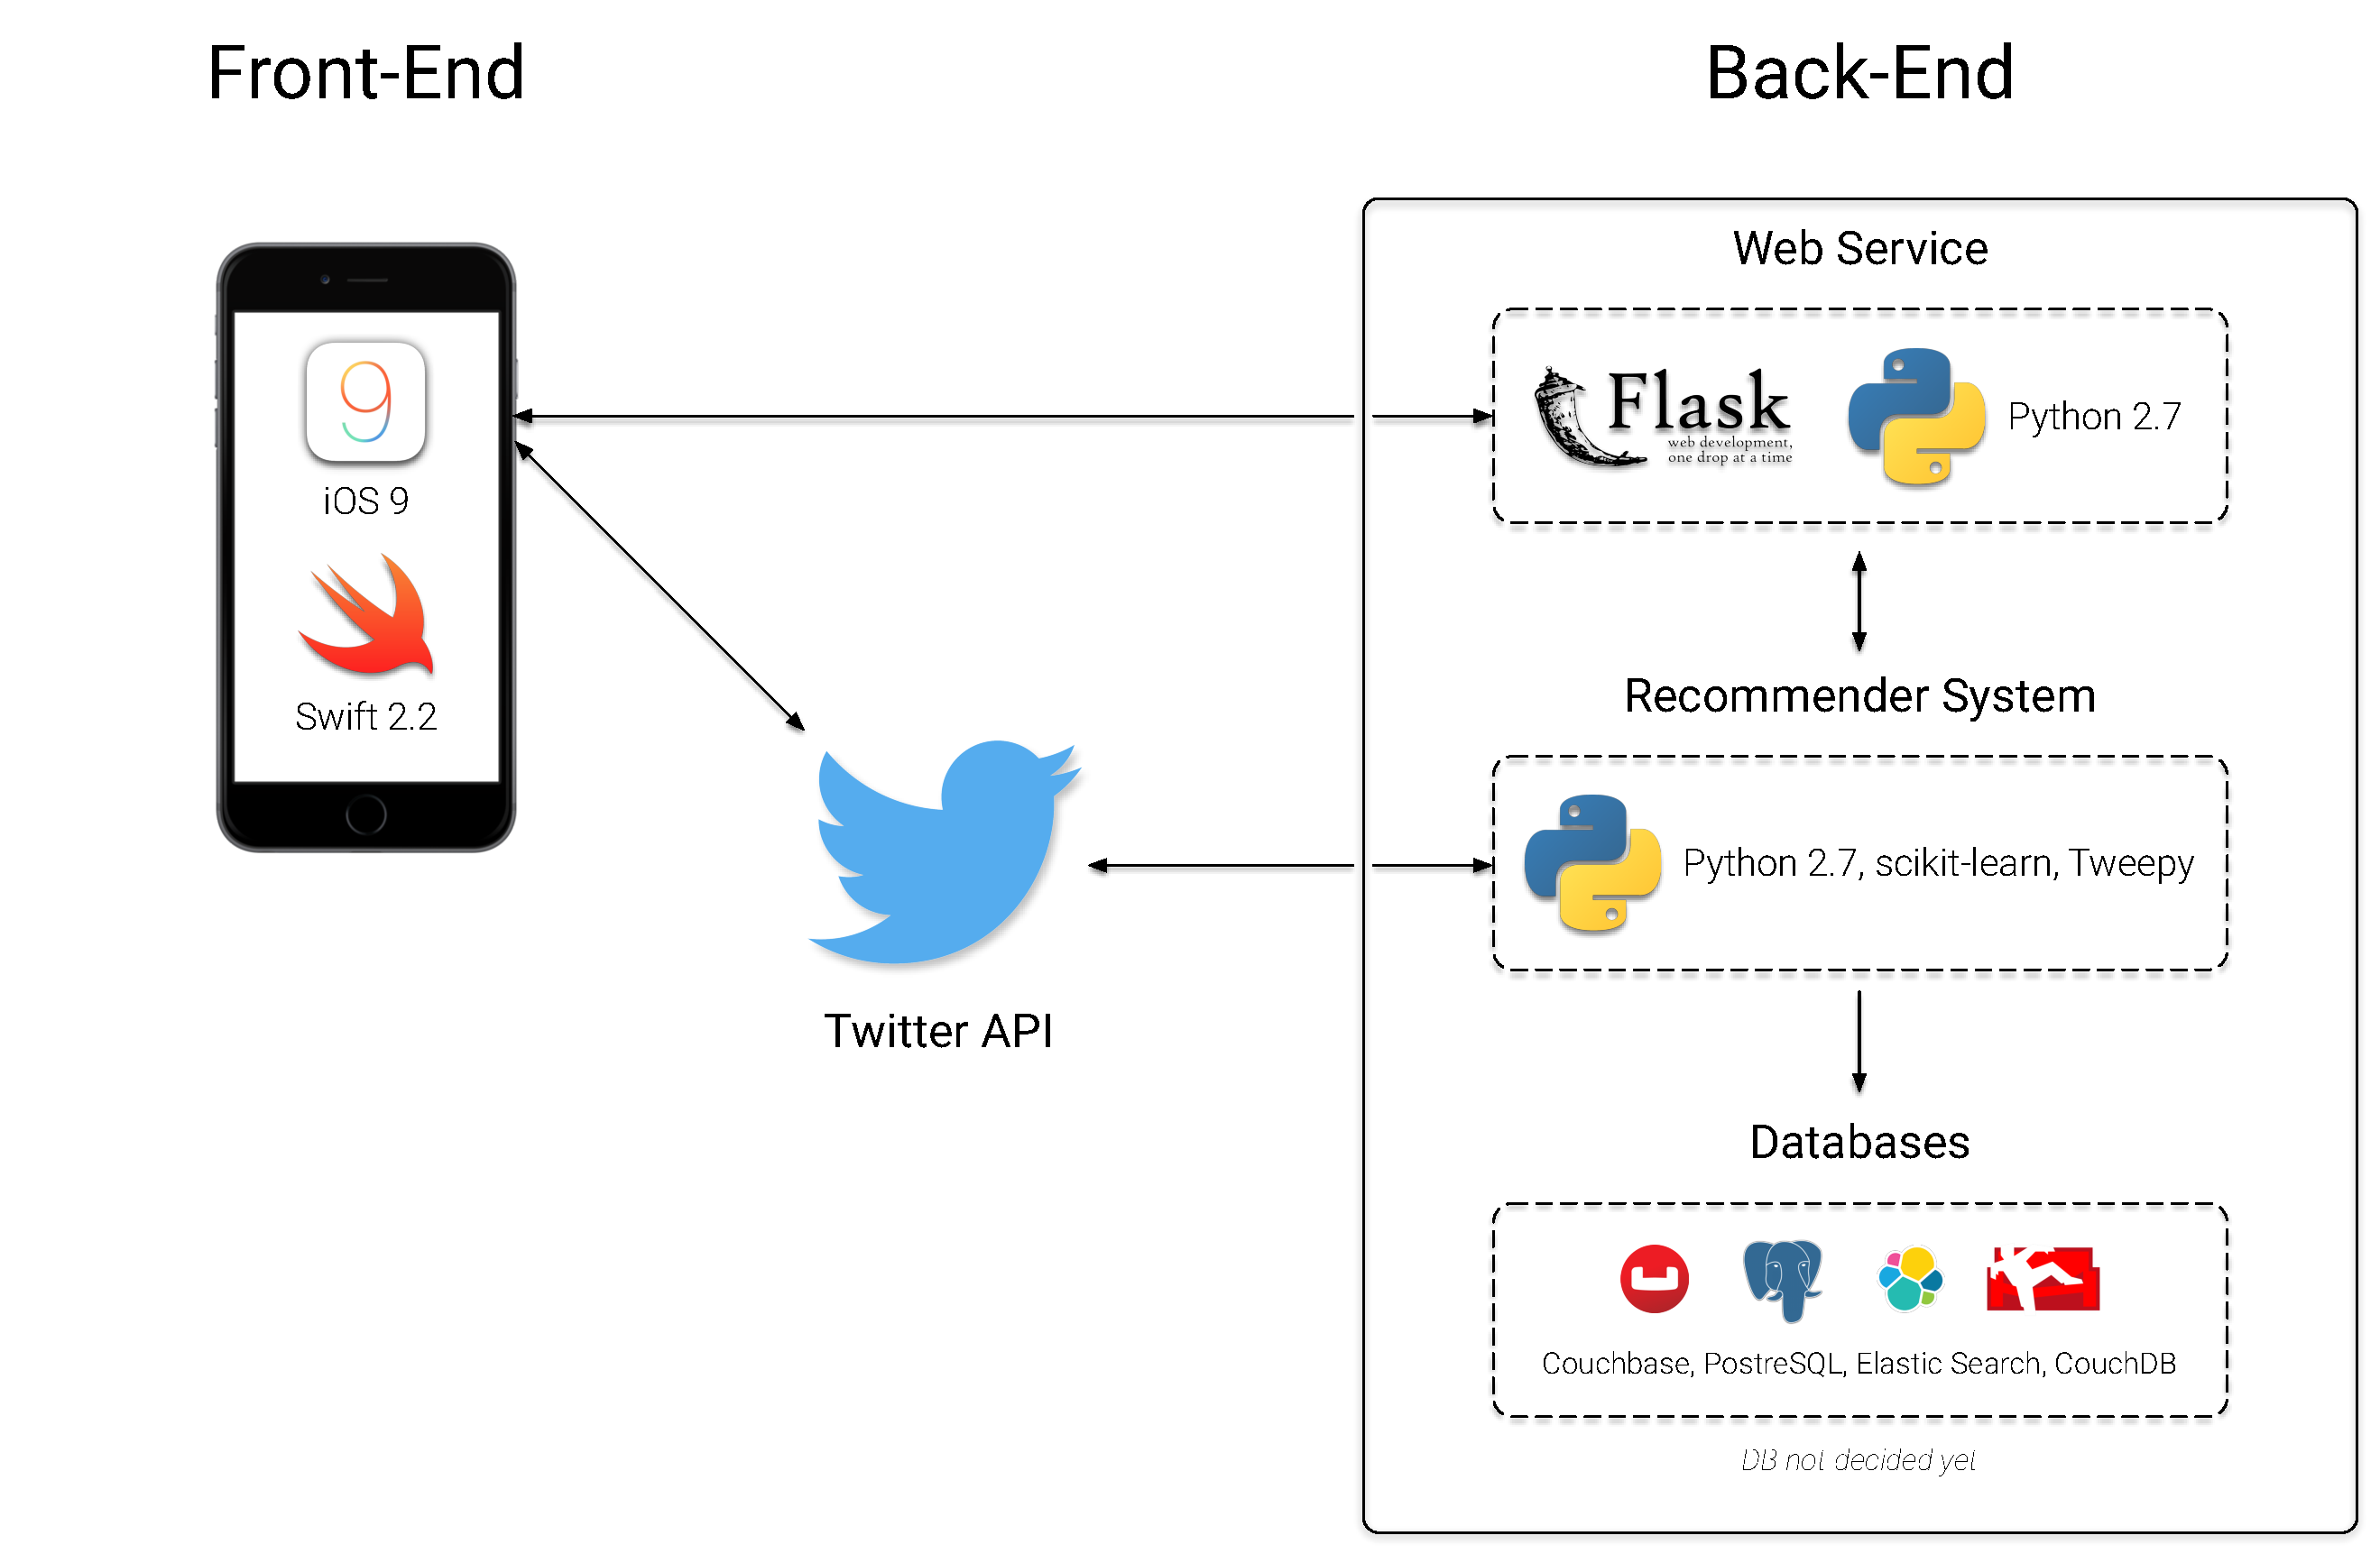
\includegraphics[width=\textwidth]{system_overview}  
    \caption{System Overview}
\end{figure}


First, the user must give the app permission to access their Twitter data. After that, the iOS client sends a request to the server.

% Comment jónsi: We may need to describe what an access token is. A non-technical
% reader is supposed to be able to follow along as he/she reads.
% This is the first time Flask is mentioned. The reader may not be familiar with 
% it or know it's a Python micro web framework.
When the server receives an iOS API request, it gets the access token which enables the server to make authorised calls to the Twitter API. Then the server uses this token to communicate with the Twitter API and fetches the user's data. Following this, the raw data is sent to the recommender system for filtering and creating recommendations. 
Lastly, the server will return the personalised tweet feed from the recommender system to the iOS client so that the user can see the personalised tweets. The colour bars on the left indicate the relevance of tweets based on the user's interests.


\newpage


\subsection{Front-End}
% Sophie: is it necessary to say when Swift was announced?
The Swift programming language was chosen as the technology used to develop the iOS client. The iOS client currently implements three functions: \hyperlink{oauth}{OAuth login}, communication with the Flask API, and Tweet data presentation.


\begin{itemize}
    \item \textbf{OAuth login}

    Because Twitter's REST API requires each request to be authorised, the system needs the users login details for their Twitter account to grant it access to the user's Twitter information. OAuth login is a complex process, so the third party library OAuthSwift \cite{oauthswift} was chosen to handle the users login process. It only requires the system to configure a few parameters, such as \textit{consumerKey} and \textit{consumerSecret}. 
    
    OAuthSwift then performs the login process, opening Twitter's website and sending a request to the Twitter authorisation API.
    Lastly, it returns the OAuth access token which is then stored on the iOS client to avoid requiring repeated logins when using the app.
 
    \item \textbf{Communication with Flask}

    Alamofire \cite{alamofire} is a popular Swift library which provides an elegant and concise way to handle HTTP network requests. The system uses it to compose dynamic HTTP requests and to append the OAuth access token to URLs. It is also used to decode JSON responses returned from the Flask server.

    \item \textbf{Tweet data presentation}
 
    After the raw JSON data is received, it needs to be converted from JSON data to a Swift primary object, like a list or dictionary. The SwiftyJSON \cite{swiftyjson} library is used to accomplish this. Then, the tweet list is hooked up to an iOS \textit{UITableView} which is a powerful iOS UI component that is suitable for displaying a list with data. The Flask server also sends weight values for each tweet, which is calculated by the recommender system to represent how much the user may like a tweet. The iOS client calculates the colour hue for the the associated weight value, which is used to set the background colour of the bar to the left of each tweet.
\end{itemize}


\newpage


\begin{figure}[H]
    \centering
    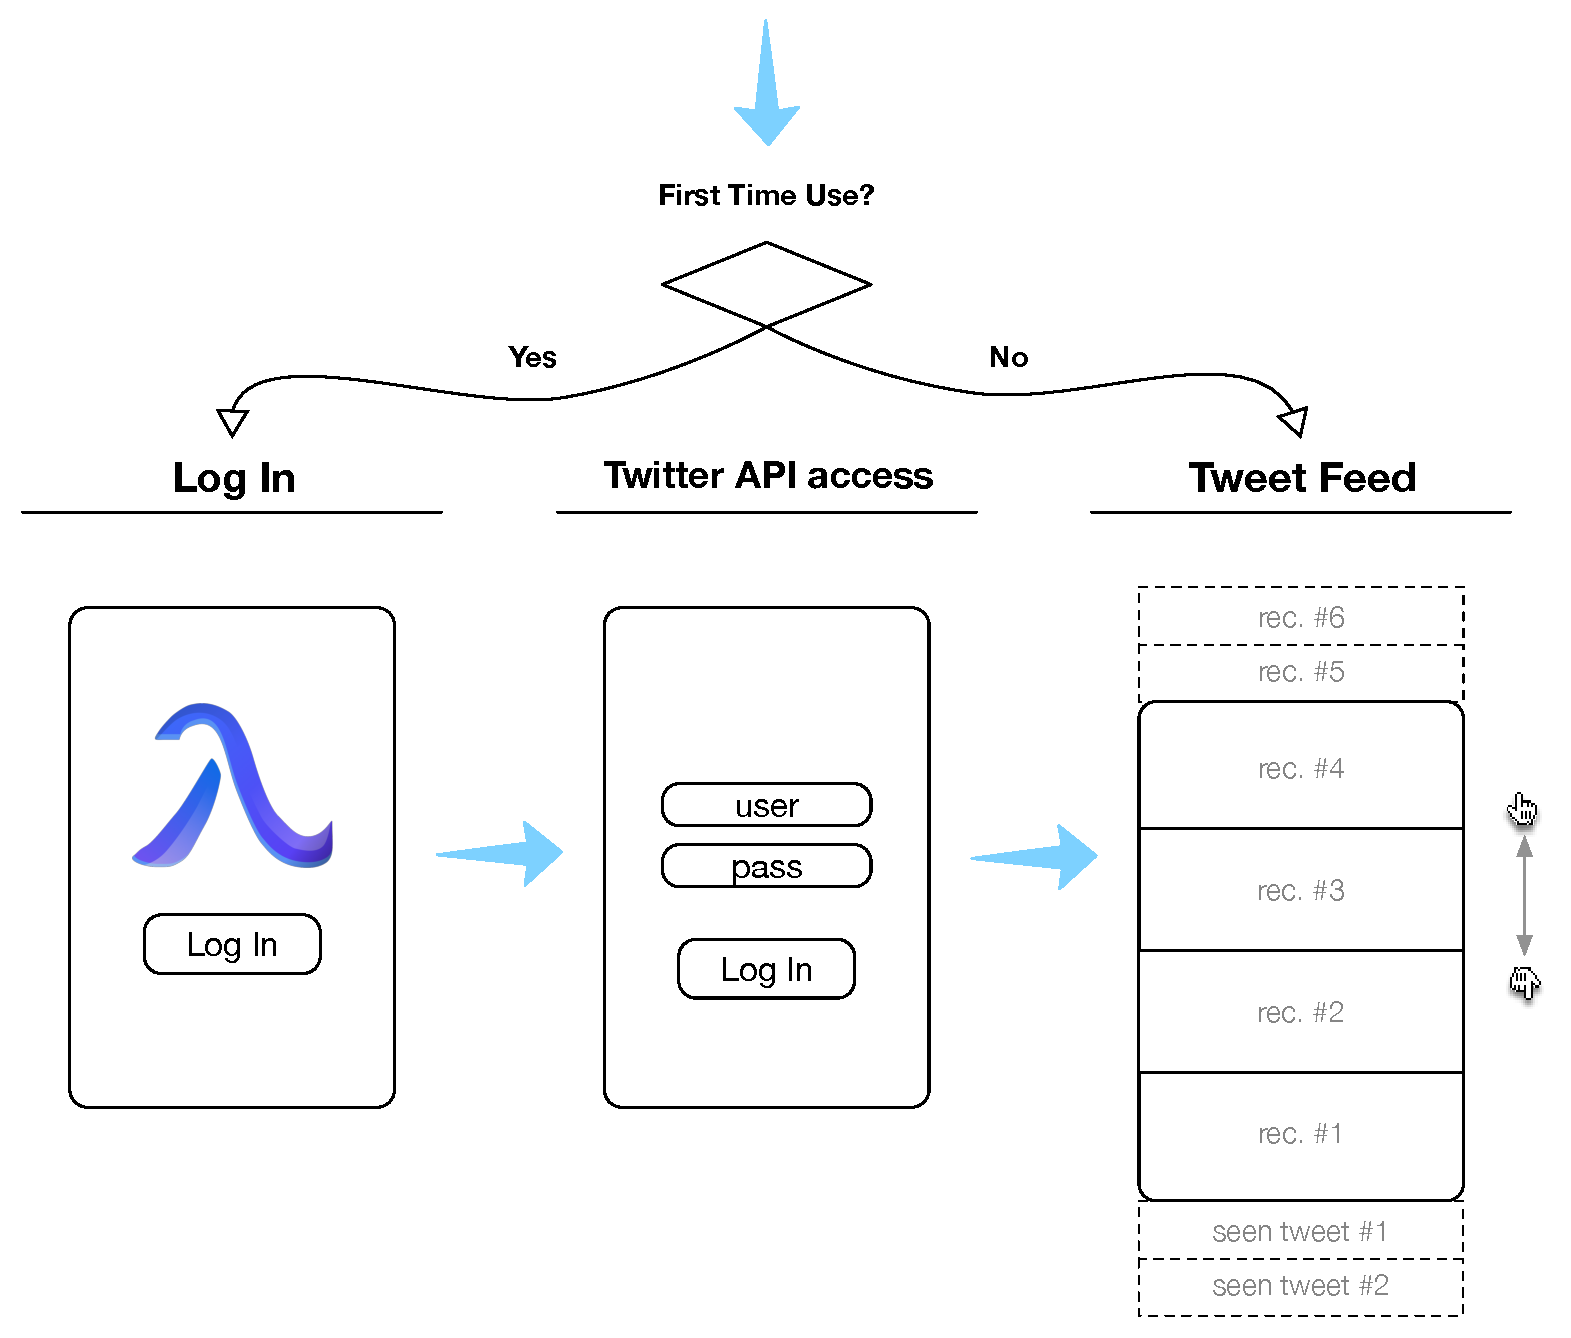
\includegraphics[width=0.78\textwidth]{ios_wireframe_1}  
    \caption{Wireframe of the flow in the iOS app}
\end{figure}

\begin{figure}[H]
    \centering
    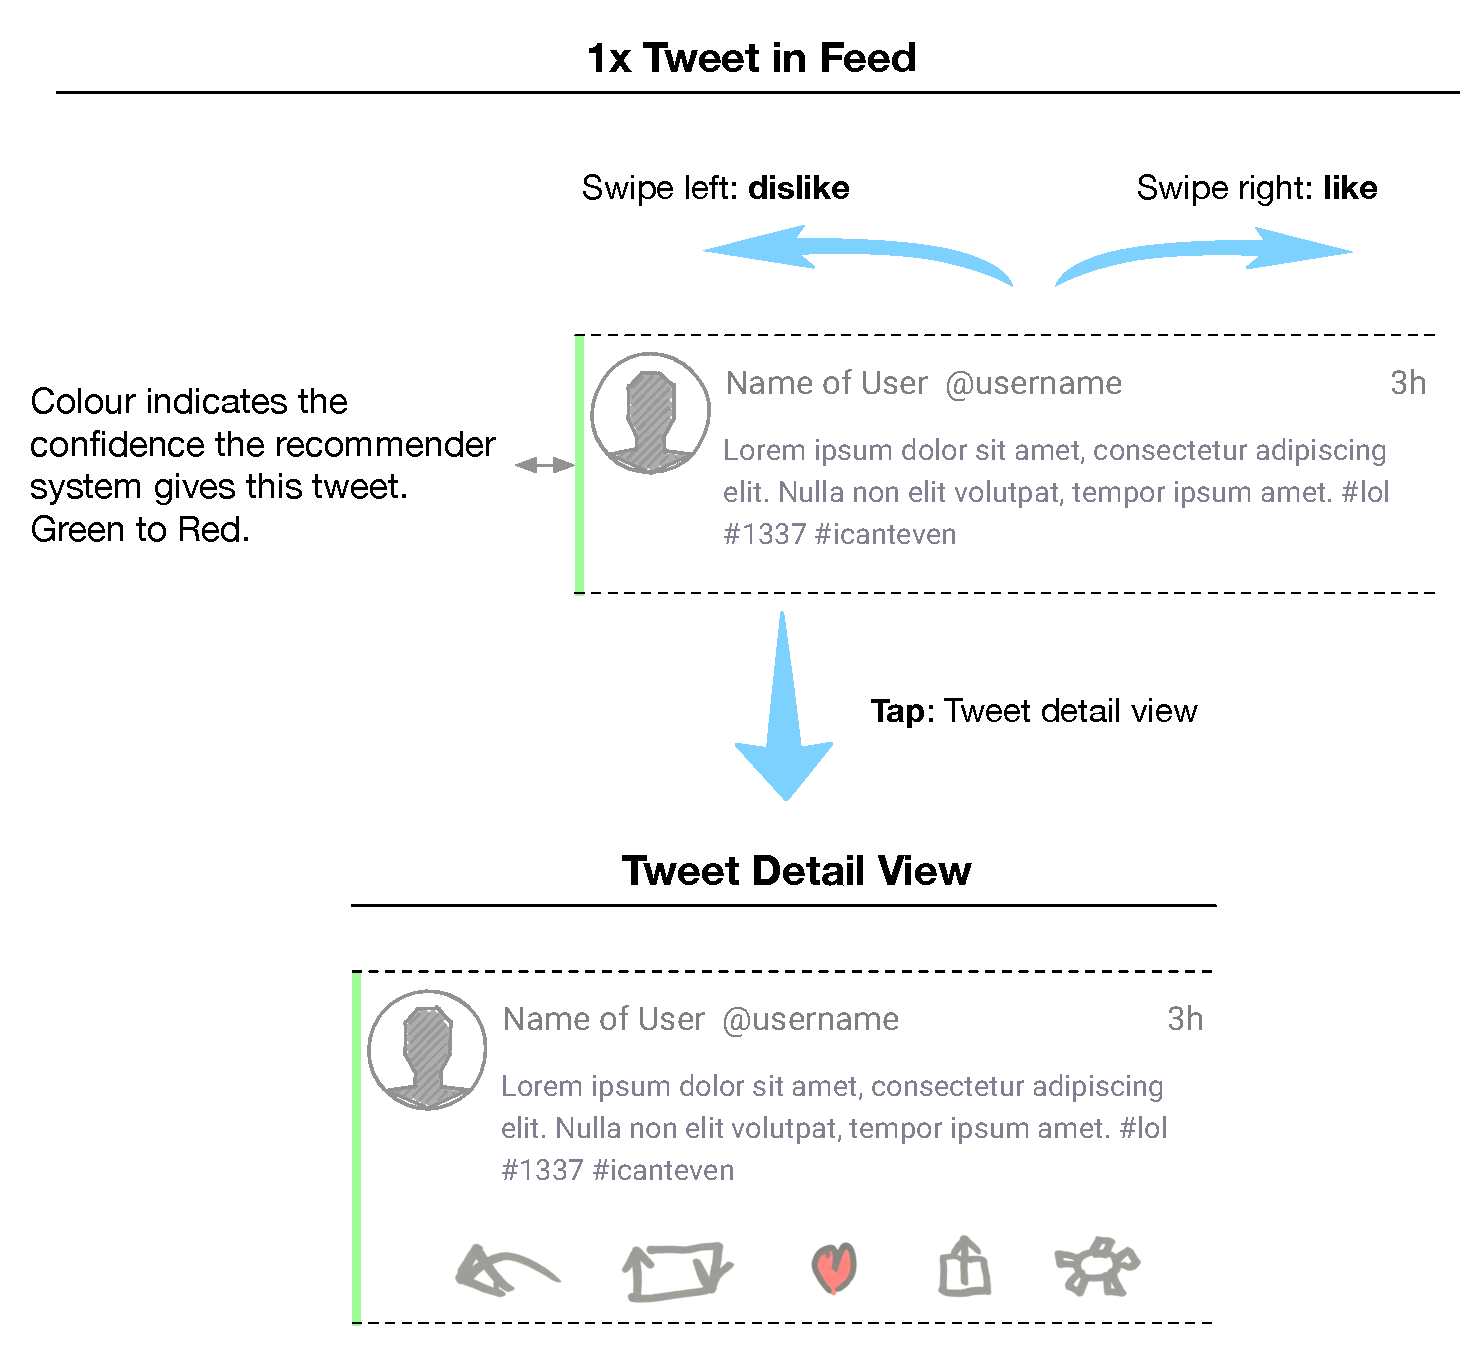
\includegraphics[width=0.78\textwidth]{ios_wireframe_2}  
    \caption{Wireframe of a Tweet in feed and detail view}
\end{figure}

\subsection{Back-End}
Our back-end consists of two parts: a web server and a recommender system. Originally Python 3.5 was used for both parts of the system, but there were compatibility issues between libraries. Due to this issue, the back-end was downgraded to Python 2.7.

For this project, three web frameworks were evaluated for the server: Django \cite{django}, Flask, and Bottle \cite{bottle}. Flask was chosen because it is more lightweight than Django and more popular and better supported (online resources, support, etc) than Bottle. Tweepy is used to interact with Twitter's APIs \cite{tweepy}.

% Maybe: a figure of the back-end components

\subsubsection*{Web Server}

The Flask Server is used to connect the iOS app and recommender system with Twitters API. Currently, it handles requests from the iOS client and fetches the user's own timeline (Tweets posted by the user), their home timeline (Tweets posted by the user and the accounts they follow) and the users profile from the Twitter API. This data is then sent to the recommender system to create tweet recommendations.

In the future, the server will also collect user gesture feedback from the iOS client and return it to the recommender system to further enhance recommendations.
\subsubsection*{Recommender System}
The recommender system is used to provide the personalised tweet home timeline for the iOS app. It performs two tasks - filtering and recommendations. 

\begin{itemize}
    \item \textbf{Filtering}

    For filtering, the recommender system filters the users home timeline by giving more relevant tweets higher priority on the timeline, while less relevant tweets are given less priority. It uses the users own tweets, likes and retweets to create a term frequency list. Then, it uses the term frequency list to place weightings (1.0 to 10.0) on each tweet that appears on the timeline. Ultimately, tweets with higher overall weightings will appear first.

    \item \textbf{Recommendations}

    For recommendations, the recommender system actively searches for popular tweets which have an abundance of retweets and likes under hashtags/words that exist in the user's term frequency list. These are found through the API via calls from the Flask server. These tweets are placed in the timeline according to their weighting accompanied by a “Follow” button, allowing the user to follow the account if they wish. An example of what this could look like in the final version of the project is as follows:
    
    \begin{center}
        
\includegraphics[width=0.6\textwidth]{follow_button}
    \end{center}

\end{itemize}

% Sophie: "unfollowed-account tweets" confused me for a while...maybe find a clearer term.
After filtering and performing recommendations, the re-ordered timeline, weighting document of tweets, and recommended tweets from non-followers will be sent to the server and returned to the iOS client. In its current build, the recommender system uses the bag-of-words approach to list the users home timeline, based on the contents of their own tweets.

\subsection{Data}
The main data source is Twitter's API, which the system uses Tweepy to access. Tweepy is easy to use and has a variety of machine learning features. For example, the Cursor\cite{cursor} object can implement the pagination of tweets in a single line of code, rather than manually using an iteration loop.

In future builds of this project, data will be required from the mobile app to refine recommendations. For example, if the user clicks a link in a tweet, likes a tweet, retweets, or otherwise engages in conversations, these events should be recorded and used to optimise the recommender system for that user. 

Further plans include having the client measure the amount of time a tweet is visible as another, more passive, observation mechanism. This will capture interest in a particular tweet, as extended time spent focusing on a single tweet likely means that the user is reading it. This could also mean that the user is simply pre-occupied elsewhere, however, and is no longer using the app. To accommodate this, different amounts of time should imply different situations. In other words, several minutes on a single tweet likely means that the user is no longer paying attention to the app, while more than a few seconds would indicate interest.
\\\\
For the MVP it was not necessary to store data, however it is one of the upcoming tasks after completion of the interim report. 

For general relational data storage PostgreSQL will probably be used. Preliminary solutions being considered to store a cache of tweets are so called document databases. Document databases are non-relational databases ideally suited to store JSON data. Since the Twitter REST API returns all data as JSON the team has confidence in that such databases will be a good fit. Databases such as Couchbase \cite{couchbase}, RethinkDB \cite{rethinkdb}, CouchDB \cite{couchdb}, and MongoDB \cite{mongodb} have been listed for further evaluation. On top of those document databases there are plans to evaluate ElasticSearch \cite{elasticsearch} to gain realtime insights into the available data.


\begin{figure}[H]
    \centering
    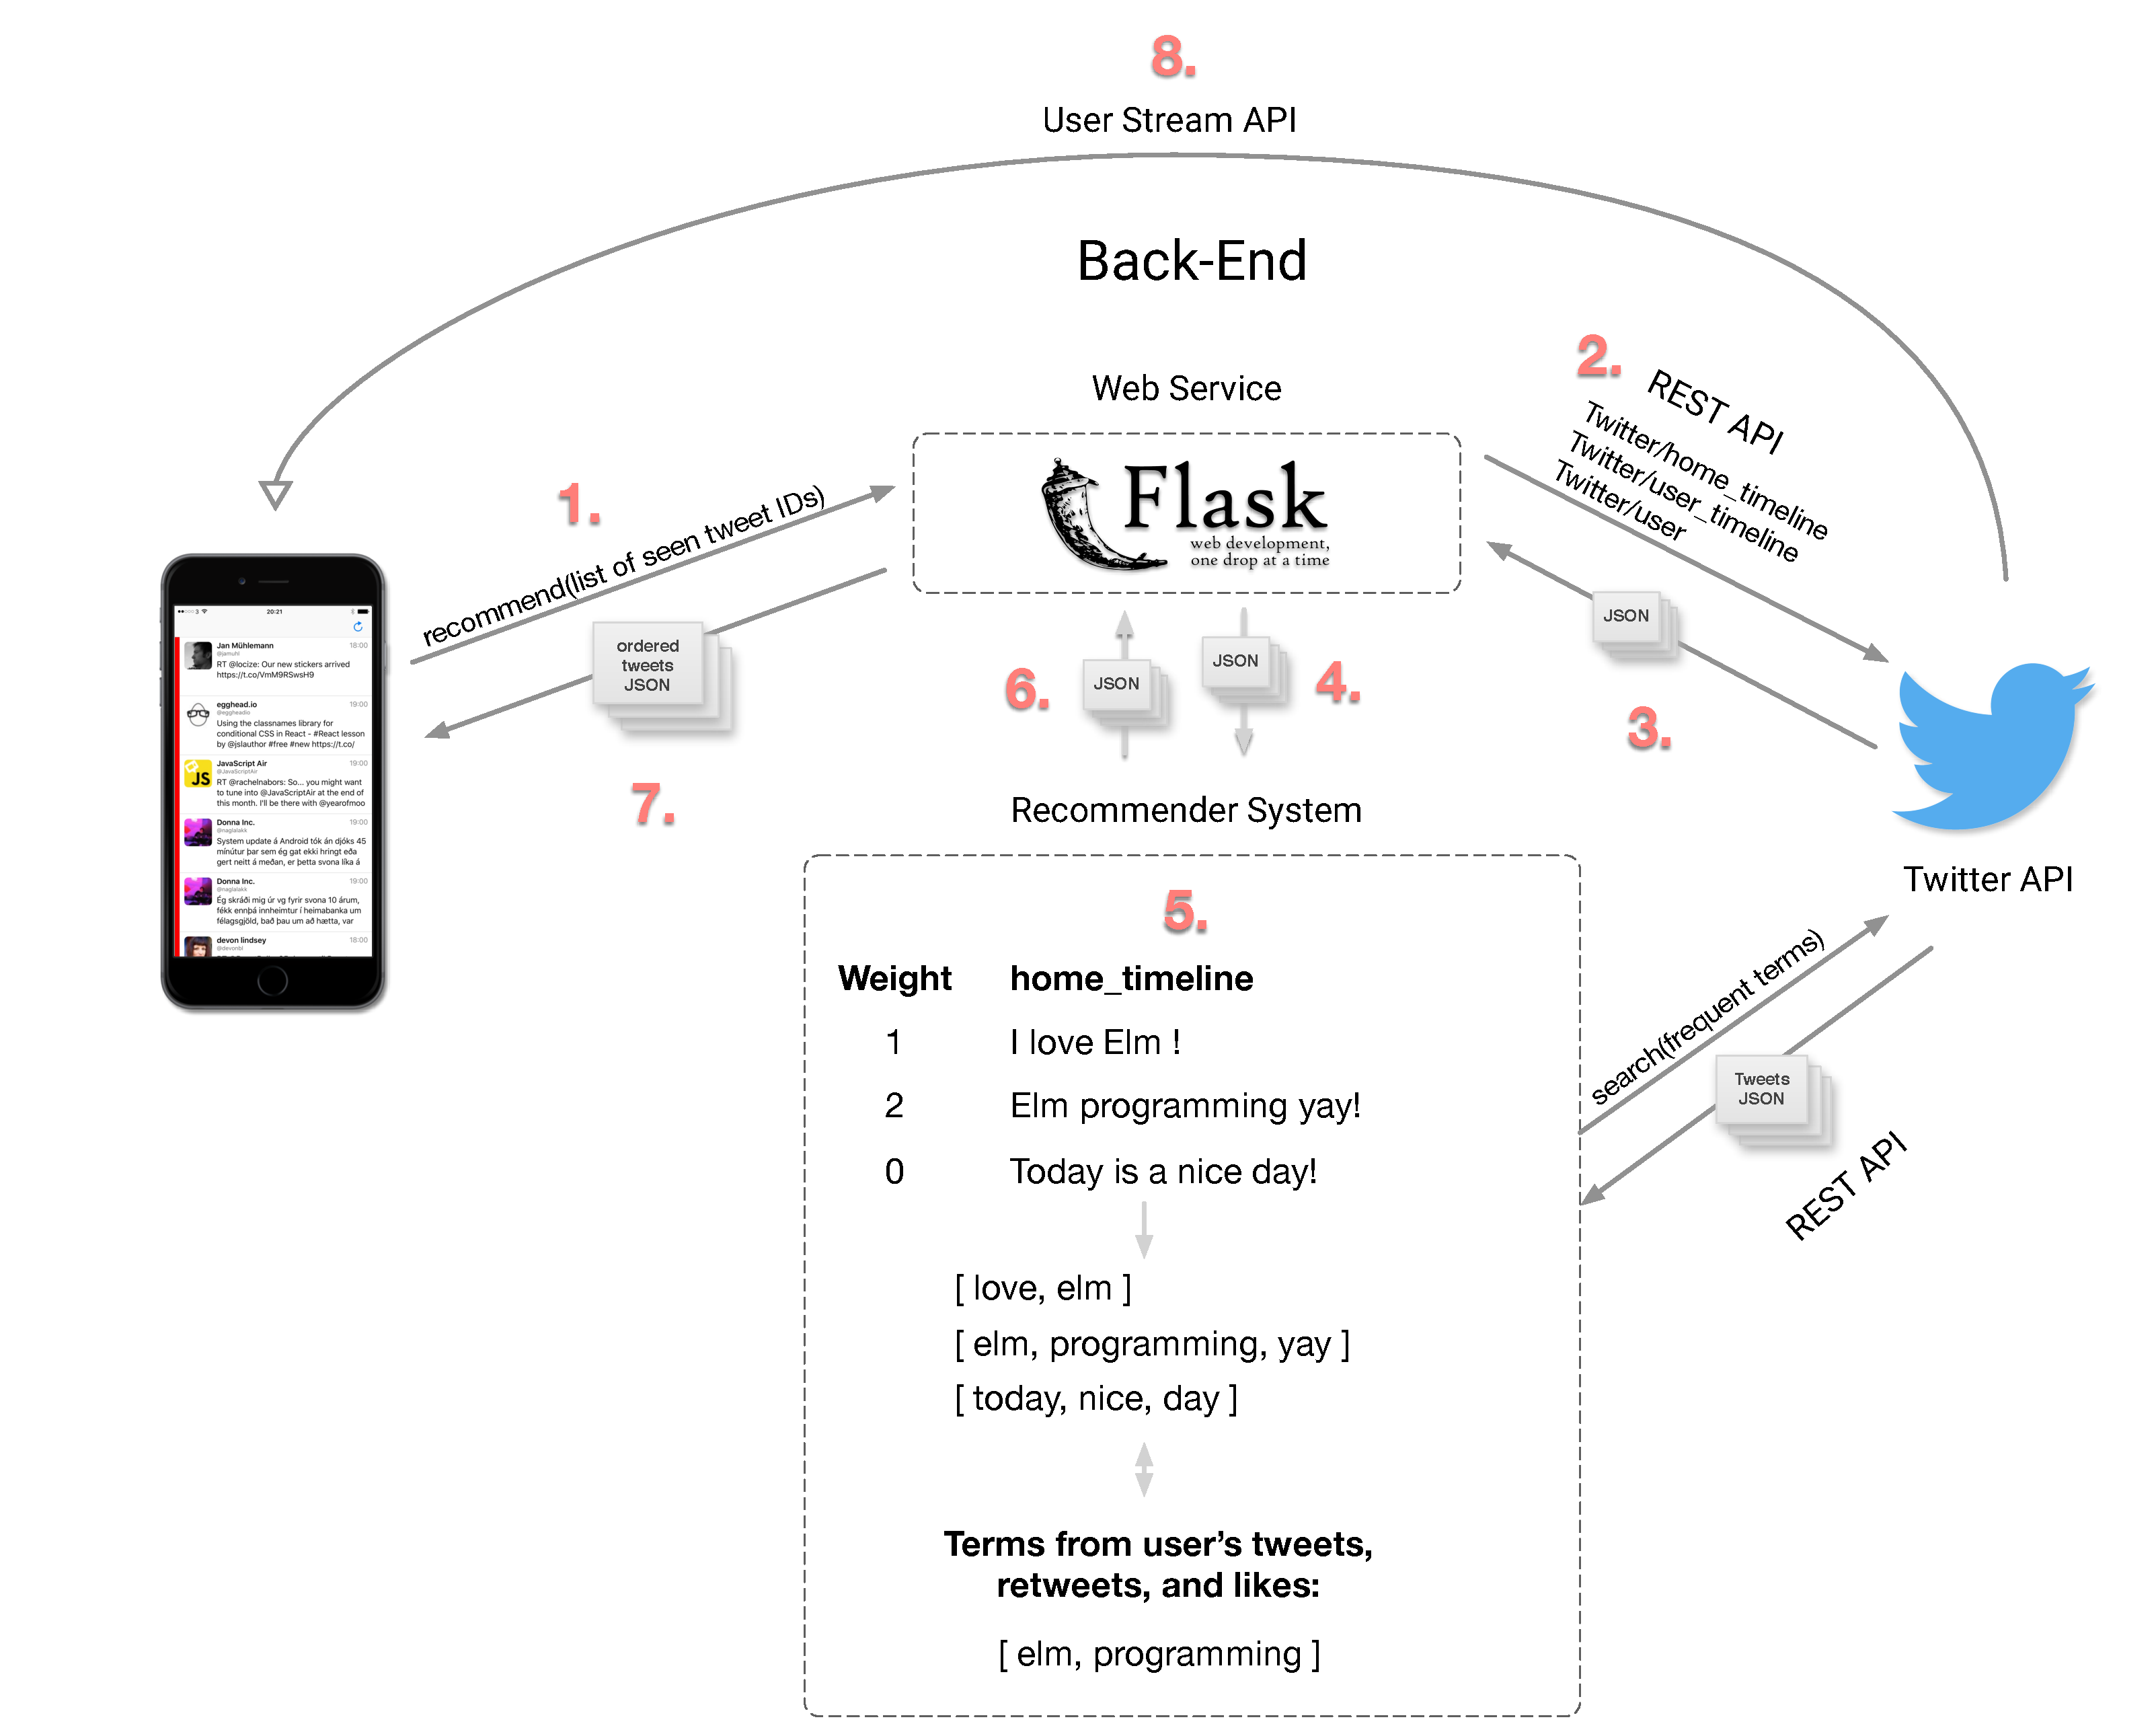
\includegraphics[width=\textwidth]{data_flow_white}  
    \caption{System Overview}
\end{figure}


\newpage


%==============================================================================
\section{Evaluation}
% 500 words, weight: 10/90 = 11%
%
% * What does success look like for your system?
% * How will you evaluate the system that you build?
%
% Grades:
%   A+ to B-: 
%		Well thought out, realistic plan for evaluation including evaluation of 
%		different aspects of the system as well as the system as a whole.
%   C+ to D-: 
%		Some thoughts on evaluation but perhaps limited to “we will ask people 
%		to use the system and tell us what they think” or very limited coverage 
%		of the system’s key components.
%    E+ to G:
%		No real evaluation plan.
%
Early observations of the MVP seemed promising when tweets from the top and bottom were compared at a glance. Although entirely subjective, it was inspiring for the team.
\\

\begin{samepage}
\noindent There are two evaluations that come to mind:

\begin{itemize*}
	\item Quality / Accuracy of the recommender system
	\item Usability and engagement in the mobile client
\end{itemize*}
\end{samepage}

\noindent A cornerstone of the project is to filter and order tweets to the user in a personalised way superior to the default Twitter feed. After the evaluation lecture by Dr. Brian Mac Namee, it was decided to focus on the recommender system as the main evaluation criteria.

Originally the intention was to benchmark the $\lambda$ Lovelace system against the recommendations that the official Twitter mobile app provides. However, investigations revealed that these recommendations are not made available in the Twitter API. The team researched and deliberated but was ultimately unable to devise any reasonable or scalable evaluation method with such restrictions. As a fallback, the system will instead be benchmarked to what is available: the users home timeline from the Twitter REST API.
\\

\begin{samepage}
\noindent Earlier evaluation method ideas included: 

\begin{itemize}
    \item Order a list of tweets by level of interest or relevancy.
    \item Present a user with a pair of tweets and ask which is more interesting or relevant: one from the $\lambda$ Lovelace system and one from the default home timeline.
\end{itemize}
\end{samepage}

\noindent In the interim presentation 2016.06.21, the team presented a tweet-pair method. However that has since been revised to the following:

\begin{figure}[H]
    \centering
    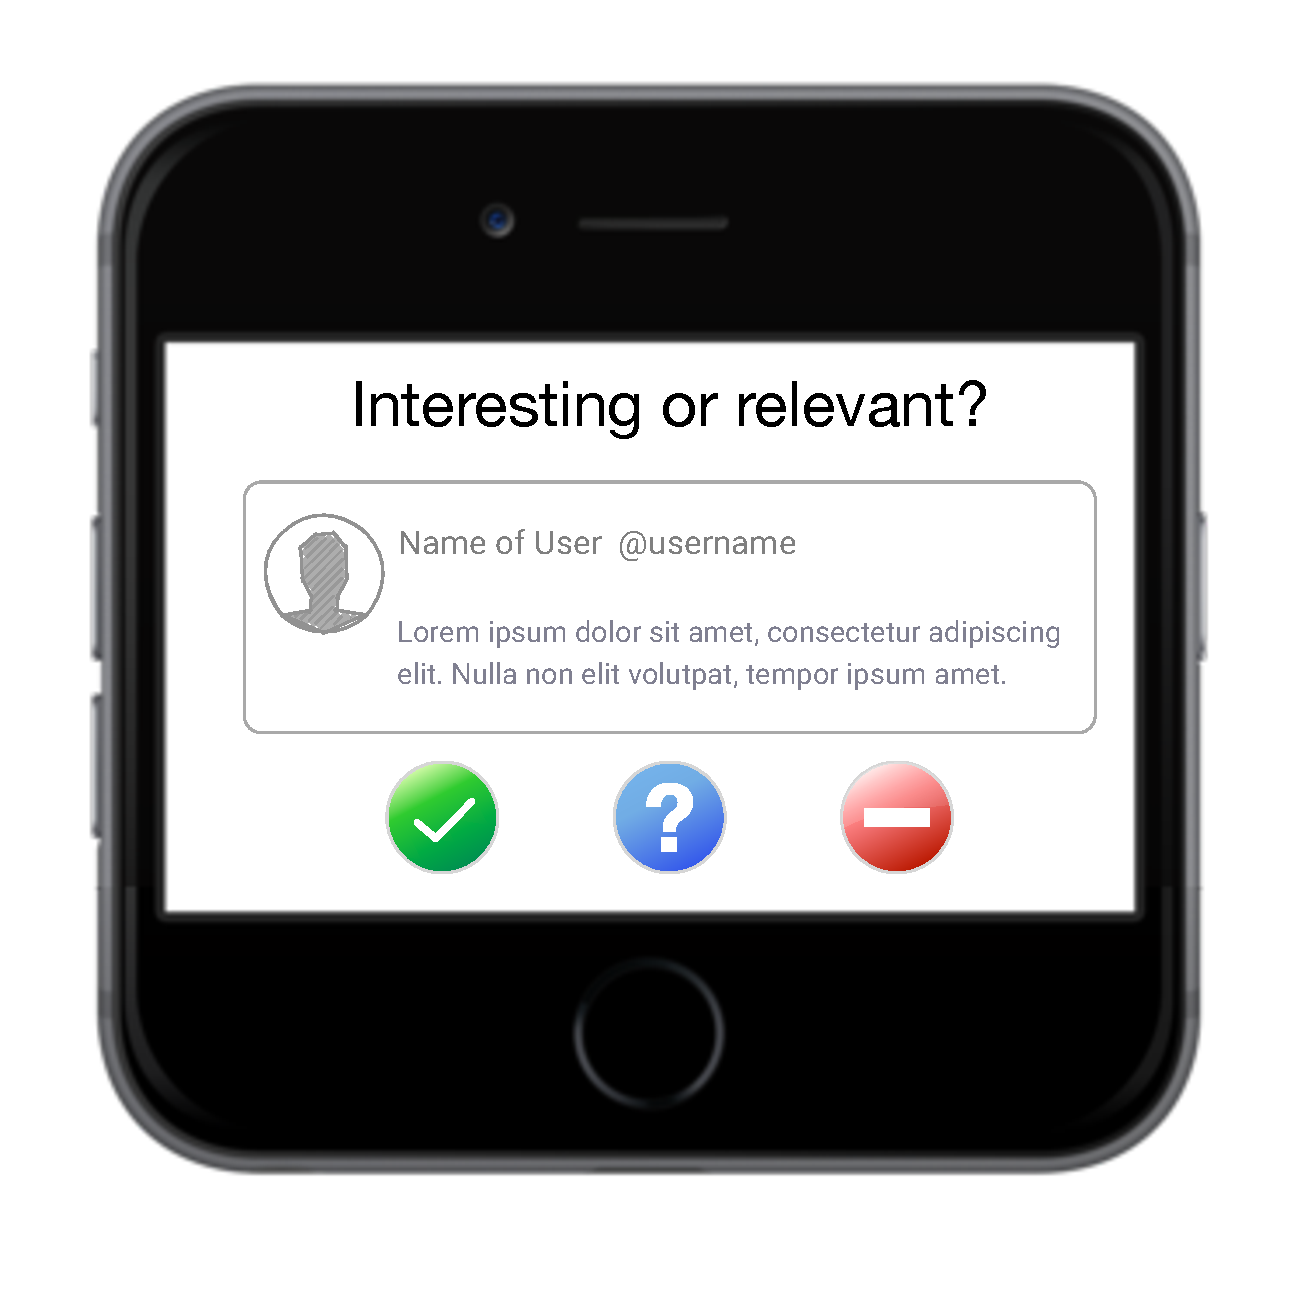
\includegraphics[width=0.45\textwidth]{tweet_evaluation}  
    \caption{A mockup of the user evaluation}
\end{figure}

\noindent The team plans to perform the evaluations in a separate view in the iOS app itself or alternatively in a specific evaluation app. This will enable re-use of much of the Swift code already written. The user will be presented with one tweet at a time and asked if he or she finds the tweet interesting or relevant. Three options are provided:

\begin{itemize*}
    \item Yes: interesting and/or relevant
    \item No: not interesting and/or not relevant
    \item Neither
\end{itemize*}

\noindent The primary motive for the switch from pair-wise tweet evaluation was to re-use and encode evaluation runs as a kind of unit test. This way, immediate feedback would be available after every change in the recommender system on all past evaluations. The state (tweets, time, etc) and results of each evaluation would persist.

\begin{figure}[H]
    \centering
    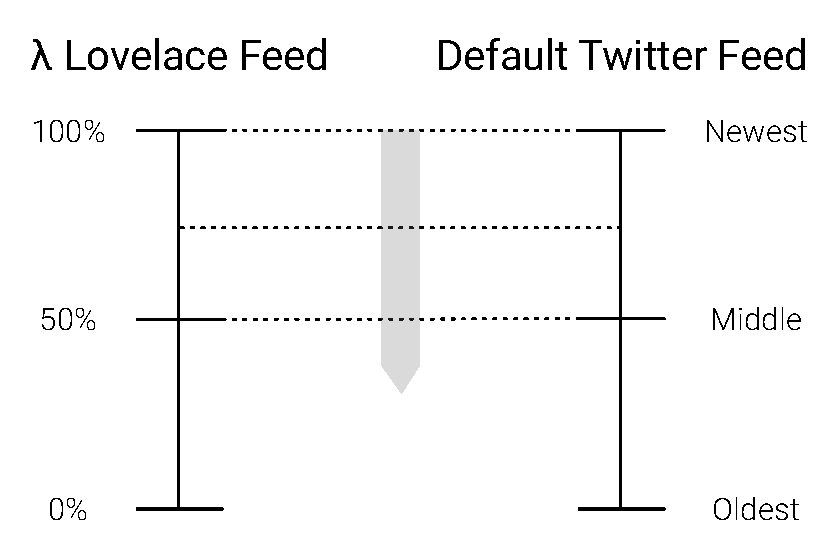
\includegraphics[width=0.6\textwidth]{evaluations_1}  
    \caption{How tweets are selected for evaluation}
\end{figure}

When an evaluation starts, tweets are picked at random from the $\lambda$ Lovelace and default Twitter feed. The user will not know from which feed the tweets came from. 50\% of the tweets will come from the $\lambda$ Lovelace feed and the other 50\% from the default Twitter chronologically-ordered home-timeline.

To benchmark the performance, votes are tallied up over all user evaluation sessions. It may be necessary to normalise each individual evaluation session because some users may find proportionally more tweets interesting or relevant than others.

\subsection{Success Definition}
We define success for this system if users will vote tweets promoted by $\lambda$ Lovelace more positively than tweets from the default Twitter, chronologically ordered home-timeline.


\newpage


%==============================================================================
\section{Conclusion: The Plan}
% 500 words, weight: 10/90 = 11%
%
% * What is your project management strategy?
% * What are the biggest challenges you are currently facing?
% * How will you use the time remaining to achieve a successful outcome?
%
% Grades:
%   A+ to B-:
%		Full description of project management plan and how this will be used 
%		to drive a successful project in the time remaining. Also clear 
%		identification of major challenges facing the project.
%  C+ to D-:
%		A plan in place for completing the project, but missing evidence of 
%		good project management or and identification of major challenges for 
%		the project.
%   E+ to G:
%		No plan in place for completing the project and little evidence of an 
%		understanding of what will be involved.
%
\subsection{Project management strategy}
The team is divided into two groups where each group is responsible for the front-end and back-end of the system. The team has has a stand-up meeting each day to encourage communication amongst members where they discuss the tasks they are currently working on, and if they are facing any "blocker" problems.

ZenHub\cite{zenhub} is used to keep track of each team members' tasks and milestones. ZenHub also gives an overall view of the team's performance using the burn-down chart functionality.

\subsection{Key Challenges}
\begin{itemize}
    \item \textbf{Twitter API rate limits}
    
    Twitter has imposed rate limits on access to their API. Each form of accessing the API, such as accessing the users home-timeline or their likes, has different rate limits. There is a 15 minute window that the limits apply to. So for a user home-timeline API call, only 15 requests are allowed in a window of 15 minutes or for a search API call only 180 requests every 15 minutes is allowed. To work around this, the project uses a database to store tweets by sending requests during these windows.
    
    \item \textbf{Home timeline limit}
    
    % Sophie: first-person "us" used here.
    Only the latest 800 tweets can be requested. This poses a problem for users that follow a lot of accounts, or for users that check Twitter very infrequently. This is the projects primary motivator to periodically collect and cache tweets in the database.
    
    \item \textbf{Evaluations in iOS client}
    
    The plan is to perform user evaluations in the iOS app itself or a separate app in order to re-use code. However some tasks remain in the iOS app, for example making sure that all types of tweets can be displayed equally well. Currently, tweets with raw text and images can be displayed. However videos, website previews and more remains to be implemented.
    
    \item \textbf{Selection of a document database}
    The need for a database did not arise while developing the MVP. For now, the team is researching which document databases are available, and which are most suitable for the $\lambda$ Lovelace system. Issues may arise here due to the teams database experience largely being restricted to relational databases. Researching and selecting a database is the next immediate step.
    
\end{itemize}


\subsection{Roadmap}
The following is a list of tasks to complete for the system within the next 5 weeks.

\begin{figure}[H]
    \centering
    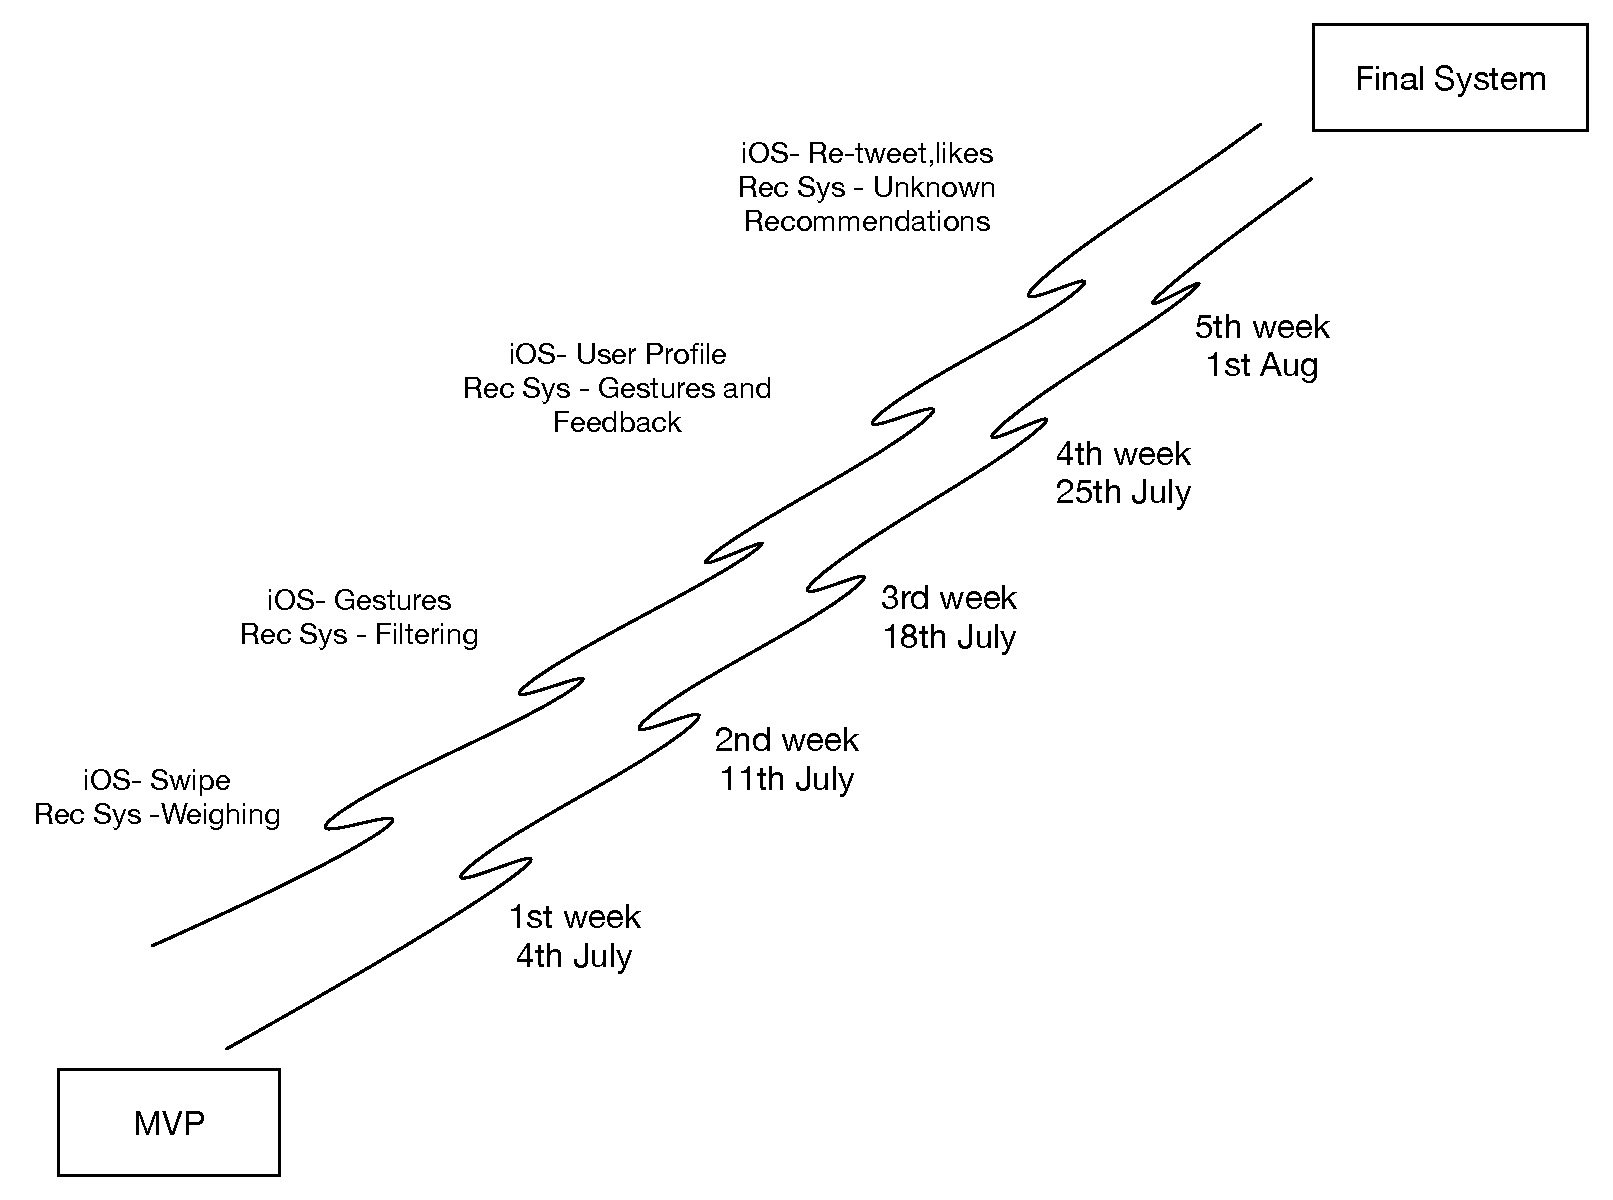
\includegraphics[width=\textwidth]{RoadMap}  
    \caption{Roadmap for future work}
\end{figure}

\newpage


%==============================================================================
\section{Appenix}
% This appendix contains information for a historical perspective such as what Twitter is and who the students and professors are. 

\subsection{Twitter Intro}
Twitter is a microblogging social network where each post or \textit{tweet} is no more than 140 characters in length. A typical Twitter user \textit{follows} multiple other users (followees) and get followed by other users (followers). By following other users they subscribe to all of their tweets and re-tweets (rebroadcast of other user's tweets). The \textit{timeline} is a chronological feed of those tweets.

\subsection{Students \& Professors}
The group project is the third and final semester of the Negotiated Learning MSc in Computer Science at University College Dublin. The students and professors involved are:
        
\begin{samepage}
\begin{center}
\begin{minipage}[t]{.4\textwidth}
	\textbf{Students}:
		\begin{itemize*}
			\item Xinqi Li
			\item Marc Laffan
			\item Junyang Ma
			\item Jón Rúnar Helgason
			\item Eazhilarasi Manivannan
		\end{itemize*}
\end{minipage}
~
\begin{minipage}[t]{.4\textwidth}
	\textbf{Module co-ordinators}:
	\begin{itemize*}
		\item Dr. Georgiana Ifrim
		\item Dr. Brian Mac Namee
		\item Dr. Derek Greene
	\end{itemize*}
\end{minipage}
\end{center}
\end{samepage}

\vspace{0.5em}

\subsection{OAuth login}
\hypertarget{oauth}
OAuth is a popular form of authentication which is used for identifying application's identity and for allowing users to grant applications access permissions. The OAuth protocol does not reveal a user's username nor password to third party applications, making it more secure than traditional authentication schemes.

\subsection{Resources}
Below are summarised lists of the resources we've utilised while working on the project: software, libraries, frameworks, tutorials, etc.

% Let's try to keep the descriptions very short, ideally the name, citation and description
% should fit on one line. It's okay to go over but this is intended to be a very high-level
% overview of what we use and for what purpose.

\subsubsection*{Front-End Swift Libraries \& Frameworks}
\begin{itemize*}
    \item \textbf{Swift} \cite{swift}: Programming language developed by Apple
    \item \textbf{iOS} \cite{ios}: Mobile operating system for the Apple iPhone and iPad
    \item \textbf{Alamofire} \cite{alamofire}: Elegant HTTP networking library
    \item \textbf{SwiftyJSON} \cite{swiftyjson}: Easier JSON data handling
    \item \textbf{OAuthSwift} \cite{oauthswift}: Swift based OAuth library for iOS
\end{itemize*}

\subsubsection*{Back-End Python Libraries \& Frameworks}
\begin{itemize*}
    \item \textbf{Flask} \cite{flask}: Micro web development framework for Python
    \item \textbf{Tweepy} \cite{tweepy}: Easy-to-use Python library for accessing the Twitter API
\end{itemize*}

\subsubsection*{Software \& Services}
\begin{itemize*}
     \item \textbf{Git} \cite{git}: Version control software for collaborative software development
     \item \textbf{Github} \cite{github}: Project hosting website that uses Git
     \item \textbf{Facebook Messenger} \cite{messenger}: Social media messaging application
     \item \textbf{Google Drive} \cite{drive}: Online storage system for documents
     \item \textbf{Zenhub} \cite{zenhub}: Chrome browser extension for Github
     \item \textbf{Omnigraffle} \cite{omnigraffle}: Graphics creation wesbite
     \item \textbf{Slack} \cite{slack}: Software-focused messaging app that integrates with Git
     \item \textbf{Pixlr} \cite{pixlr}: Online image editor
     \item \textbf{ShareLaTeX} \cite{sharelatex}: Collaborative LaTeX environment
     \item \textbf{Celery} \cite{celery}: Asynchronous job queuing software
\end{itemize*}

\subsubsection*{Learning Resources}
\begin{itemize*}
    \item \textbf{Python Cookbook} \cite{cookbook}: An intermediate-level Python textbook.
    \item \textbf{Python 3 Essential Training} \cite{lynda}: A Lynda.com online training course.
\end{itemize*}


\newpage


%==============================================================================
% References
% 
% List of resources: software, papers, tutorials, books. 
%
%==============================================================================
\begin{thebibliography}{9} 

\bibitem {clark1}
    Andrew Clark Tweet One \\
    \url{https://twitter.com/acdlite/status/745345694949507072}
    
\bibitem {clark2}
    Andrew Clark Tweet Two \\
    \url{https://twitter.com/acdlite/status/745273848233230337}
    
\bibitem {ll-blog}
	$\lambda$ Lovelace blog, \url{https://jonrh.github.io/lambda-lovelace/}
	
\bibitem {ucdgithub}
	Negotiated Learning Project organisation on GitHub \\
	\url{https://github.com/ucd-nlmsc-teamproject}

\bibitem {swift}
	Swift official website \url{https://developer.apple.com/swift/}
	
\bibitem {ios}
	iOS official website \url{http://www.apple.com/ie/ios/}

\bibitem {gitrepo}
	$\lambda$ Lovelace code repository on GitHub \\
	\url{https://github.com/jonrh/lambda-lovelace/}
	
\bibitem {zenhub}
	ZenHub official website \url{https://www.zenhub.com/}

\bibitem {flask}
    Flask project website \url{http://flask.pocoo.org/}
    
\bibitem {git}
    Git website \url{https://git-scm.com/}

\bibitem {github}
    Github website \url{https://github.com/}

\bibitem {messenger}
    Facebook Messenger \url{https://www.messenger.com/}

\bibitem {drive}
    Google Drive website \url{https://www.google.ie/drive/}

\bibitem {omnigraffle}
    Omnigraffle website \url{https://www.omnigroup.com/omnigraffle}

\bibitem {slack}
    Slack website \url{https://slack.com/}
    
\bibitem {pixlr}
    Pixlr website \url{https://pixlr.com/}
     
\bibitem {sharelatex}
    ShareLaTeX website \url{https://www.sharelatex.com}
    
\bibitem {celery}
    Celery website \url{http://www.celeryproject.org/}

\bibitem {Swift}
    Swift website \url{https://developer.apple.com/swift/}
    
\bibitem {oauthswift}
    OAuthSwift GitHub repository \\
    \url{https://github.com/OAuthSwift/OAuthSwift}
    
\bibitem {alamofire}
    Alamofire GitHub repository \\
    \url{https://github.com/Alamofire/Alamofire}
    
\bibitem {swiftyjson}
    SwiftyJSON GitHub repository \\
    \url{https://github.com/SwiftyJSON/SwiftyJSON}
    
\bibitem {django}
    Django project website \url{https://www.djangoproject.com/}
    
\bibitem {bottle}
    Bottle project website \url{http://bottlepy.org/docs/dev/index.html}
    
\bibitem {tweepy}
    Tweepy GitHub repository \url{https://github.com/tweepy/tweepy}

\bibitem {cursor}
    Tweepy Cursor Tutorial \\ 
    \url{http://tweepy.readthedocs.io/en/v3.5.0/cursor_tutorial.html}
    
\bibitem {couchbase}
    Couchbase \url{http://www.couchbase.com/}
    
\bibitem {rethinkdb}
    RethinkDB \url{http://rethinkdb.com/}

\bibitem {couchdb}
    CouchDB \url{http://couchdb.apache.org/}

\bibitem {mongodb}
    MongoDB \url{https://www.mongodb.com/}

\bibitem {elasticsearch}
    ElasticSearch \url{https://www.elastic.co/products/elasticsearch}
    
\bibitem {cookbook}
    Python Cookbook \\
    \url{http://shop.oreilly.com/product/0636920027072.do}
    
\bibitem {lynda}
    Python 3 Essential Training \\ \url{https://www.lynda.com/Python-3-tutorials/essential-training/62226-2.html}

\end{thebibliography}


\newpage

\end{document}